\documentclass[11pt]{article}

\usepackage{amsmath,amssymb,mathtools}
\usepackage[margin=1in]{geometry}
\usepackage{enumitem}
\usepackage{xcolor}
\usepackage{microtype}
\usepackage{graphicx}
\usepackage{tikz,float}
\usepackage{subcaption}
\usepackage{amsthm}
\usepackage{hyperref}
\usepackage{array}
\usepackage{pgfplots}

\usetikzlibrary{shapes.geometric, arrows.meta, positioning, calc, decorations.markings}
\tikzset{
	block/.style={rectangle, draw, text width=6em, text centered, rounded corners, minimum height=10mm},
	sum/.style={circle, draw, node distance=1.5cm},
	line/.style={draw, -{Stealth[length=2.5mm, width=1.5mm]}}
}

\usepgfplotslibrary{groupplots}
\pgfplotsset{compat=1.18}

\pgfplotsset{
	myaxes/.style={
		axis lines=middle,
		axis line style={-latex},
		grid=major,
		grid style={gray!15},
		minor grid style={gray!35},
		xlabel style={at={(ticklabel* cs:1)}, anchor=north west},
		ylabel style={at={(ticklabel* cs:1)}, anchor=south east},
		every axis plot/.append style={thick}
	},
	myplotstyle/.style={
		width=14cm,
		height=7cm,
		axis lines=middle,
		axis line style={-Stealth},
		grid=both,
		minor tick num=1,
		major grid style={draw=gray!30},
		minor grid style={draw=gray!15},
		tick label style={font=\small, fill=white, inner sep=1.5pt},
		xlabel={$t$},
		ylabel={$x(t)$},
		xlabel style={anchor=north east, font=\small},
		ylabel style={anchor=south east, font=\small},
		samples=401,
	}
}

\newtheoremstyle{mynote}
{6pt}      % Space above
{6pt}      % Space below
{}          % Body font (normal, not italic)
{}          % Indent amount
{\bfseries} % Theorem head font
{.}         % Punctuation after theorem head
{.5em}      % Space after theorem head
{}          % Theorem head spec
\theoremstyle{mynote}
\newtheorem{definition}{Definition}
\newtheorem{proposition}{Proposition}
\newtheorem{example}{Example}
\newtheorem{remark}{Remark}
\newtheorem{theorem}{Theorem}
\newtheorem{corollary}{Corollary}

\newcommand{\T}{\mathcal{T}}
\newcommand{\R}{\mathbb{R}}
\newcommand{\Z}{\mathbb{Z}}
\newcommand{\C}{\mathbb{C}}
\newcommand{\conv}{\ast}
\newcommand{\dt}{\,\dd t}
\newcommand{\dd}{\mathrm{d}}
\newcommand{\imp}{\delta}
\newcommand{\sinc}[1]{\frac{\sin(\pi #1)}{\pi #1}}


\DeclareMathOperator{\rect}{rect}
\DeclareMathOperator{\Ev}{Ev}
\DeclareMathOperator{\Od}{Od}
\DeclareMathOperator{\sgn}{sgn}
\DeclareMathOperator{\step}{u}
\DeclareMathOperator{\tri}{tri}


\begin{document}
	% Reset figure counter for this lecture
	\renewcommand{\thefigure}{3.\arabic{figure}}
	
	% --- TITLE BLOCK ---
	\thispagestyle{empty}
	\noindent
	\begin{tabular*}{\textwidth}{l @{\extracolsep{\fill}} r}
		\textbf{Signals and Systems} & \textbf{Lecture 3} \\
		\textit{Dr. Ghandi Manasra and Ahmed Rabei} & \textit{Fall 2025} \\
	\end{tabular*}
	\hrule
	\vspace{0.4cm}
	\begin{center}
		\Large\textbf{Lecture 3: Systems and Their Properties}
	\end{center}
	\vspace{0.4cm}
	
\section*{Reference}
	Oppenheim \& Willsky, \textit{Signals and Systems}, Chapter 1, Sections 1.5--1.6; MIT OCW lecture notes on LTI systems.

	\section*{Review of Lecture 2}
	\begin{itemize}[noitemsep]
		\item Elementary signals toolbox introduced
		\item Unit impulse sifting property
		\item Signal representation building blocks
		\item Today: systems and properties
	\end{itemize}
	
	\section*{3.1 Systems and Interconnections}
	
	A \textbf{system} is any process that transforms an input signal into an output signal. It can be modeled by an operator \(\T\{\cdot\}\) mapping an input signal to an output signal:
	\[
	\text{Continuous-Time (CT):} \quad y(t) = \T\{x(t)\}, \qquad \text{Discrete-Time (DT):} \quad y[n] = \T\{x[n]\}.
	\]
	\begin{figure}[H]
		\centering
		\begin{subfigure}[b]{0.48\textwidth}
			\centering
			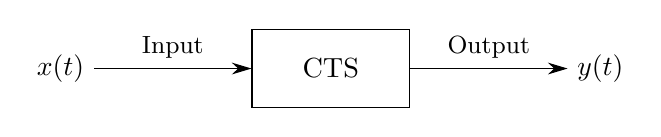
\begin{tikzpicture}[node distance=2cm, auto, >=Stealth]
	% Node for the system block (black and white)
	\node[draw, rectangle, minimum width=2cm, minimum height=1cm, text width=5em, text centered] (system) {CTS};
	
	% Input and Output nodes
	\node (input) [left=of system] {$x(t)$};
	\node (output) [right=of system] {$y(t)$};
	
	% Connecting lines with labels (black)
	\path[line] (input) -- node[above, font=\small] {Input} (system);
	\path[line] (system) -- node[above, font=\small] {Output} (output);
\end{tikzpicture}
			\caption{Continuous-Time System}
			\label{fig:ct_system}
		\end{subfigure}
		\hfill
		\begin{subfigure}[b]{0.48\textwidth}
			\centering
			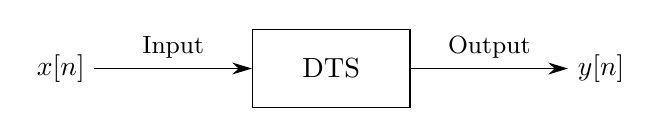
\begin{tikzpicture}[node distance=2cm, auto, >=Stealth]
	% Node for the system block (black and white)
	\node[draw, rectangle, minimum width=2cm, minimum height=1cm, text width=5em, text centered] (system) {DTS};
	
	% Input and Output nodes
	\node (input) [left=of system] {$x[n]$};
	\node (output) [right=of system] {$y[n]$};
	
	% Connecting lines with labels (black)
	\path[line] (input) -- node[above, font=\small] {Input} (system);
	\path[line] (system) -- node[above, font=\small] {Output} (output);
\end{tikzpicture}
			\caption{Discrete-Time System}
			\label{fig:dt_system}
		\end{subfigure}
		\caption{Continuous-time and discrete-time system blocks.}
		\label{fig:system_blocks}
	\end{figure}
	
	Systems are often interconnected to compose complex processing chains. Common interconnections include:
	\begin{enumerate}[noitemsep]
		\item \textbf{Series (Cascade):} Output of \(\T_1\) feeds input of \(\T_2\).
		\item \textbf{Parallel:} Same input fed to multiple systems; outputs summed.
		\item \textbf{Feedback:} Output fed back to the input and combined with the original input.
	\end{enumerate}
	
	\begin{figure}[H]
		\centering
		
\usetikzlibrary{positioning}

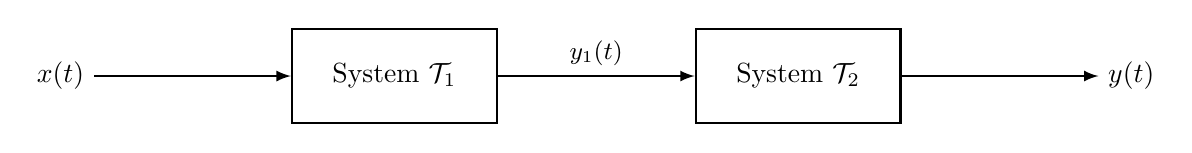
\begin{tikzpicture}[
	% Set the default distance between nodes.
	node distance=1.5cm and 2.5cm
	]
	% Define custom styles to make the code cleaner and more reusable.
	\tikzset{
		block/.style={draw, rectangle, minimum height=1.2cm, minimum width=2.6cm, align=center, thick},
		line/.style={-latex, thick} % Use -latex for a nicer arrowhead
	}
	
	% === NODES ===
	% Place the nodes for the diagram, from left to right.
	
	\node (input) {\(x(t)\)};
	\node[block, right=of input] (sys1) {System \(\mathcal{T}_1\)};
	\node[block, right=of sys1] (sys2) {System \(\mathcal{T}_2\)};
	\node[right=of sys2] (output) {\(y(t)\)};
	
	% === CONNECTIONS ===
	% Draw the lines and arrows connecting the nodes.
	
	\draw[line] (input) -- (sys1);
	\draw[line] (sys1) -- node[midway, above, font=\small] {\(y_1(t)\)} (sys2);
	\draw[line] (sys2) -- (output);
\end{tikzpicture}
		\caption{Series cascade interconnection example.}
		\label{fig:series}
	\end{figure}
	
	\begin{figure}[H]
		\centering
		
\usetikzlibrary{positioning}

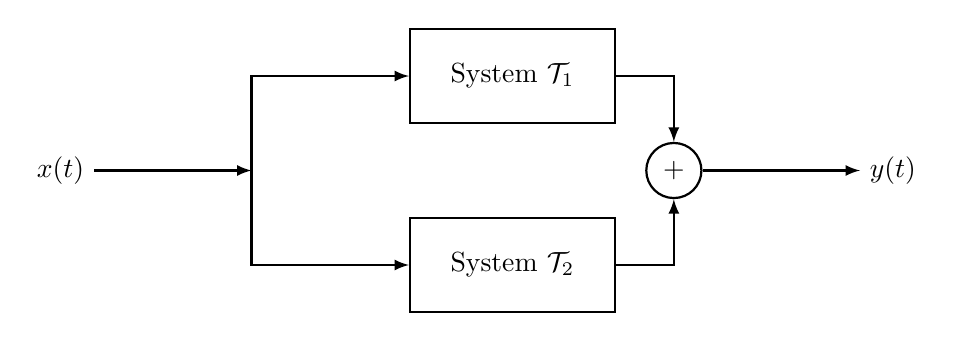
\begin{tikzpicture}[
	% Set the default distance between nodes.
	node distance=1.5cm and 2cm
	]
	% Define custom styles to make the code cleaner and more reusable.
	\tikzset{
		block/.style={draw, rectangle, minimum height=1.2cm, minimum width=2.6cm, align=center, thick},
		sum/.style={draw, circle, inner sep=0pt, minimum size=7mm, thick},
		line/.style={-latex, thick} % Use -latex for a nicer arrowhead
	}
	
	% === NODES ===
	% Place the nodes for the diagram, starting from the left.
	
	\node (input) {\(x(t)\)};
	\node[coordinate, right=of input] (split) {};
	\node[block, right=of split, yshift=1.2cm] (sys1) {System \(\mathcal{T}_1\)};
	\node[block, right=of split, yshift=-1.2cm] (sys2) {System \(\mathcal{T}_2\)};
	\node[sum, right=5cm of split] (summer) {\(+\)};
	\node[right=of summer] (output) {\(y(t)\)};
	
	% === CONNECTIONS ===
	% Draw the lines and arrows connecting the nodes.
	
	\draw[line] (input) -- (split);
	\draw[line] (split) |- (sys1.west);
	\draw[line] (split) |- (sys2.west);
	\draw[line] (sys1.east) -| (summer.north);
	\draw[line] (sys2.east) -| (summer.south);
	\draw[line] (summer) -- (output);
\end{tikzpicture}

		\caption{Parallel interconnection example.}
		\label{fig:parallel}
	\end{figure}
	
	\begin{figure}[H]
		\centering
		
\usetikzlibrary{positioning}

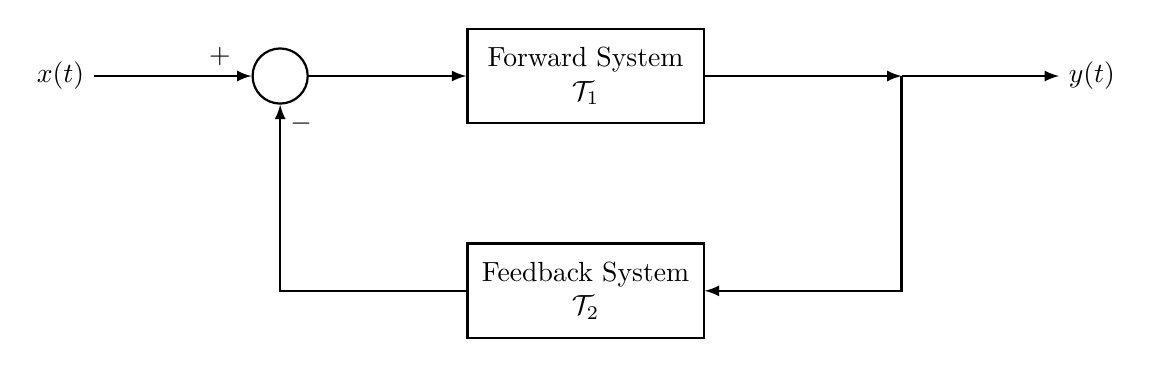
\begin{tikzpicture}[
	% Set the default distance between nodes.
	node distance=1.5cm and 2cm
	]
	% Define custom styles to make the code cleaner and more reusable.
	\tikzset{
		block/.style={draw, rectangle, minimum height=1.2cm, minimum width=3cm, align=center, thick},
		sum/.style={draw, circle, inner sep=0pt, minimum size=7mm, thick},
		line/.style={-latex, thick} % Use -latex for a nicer arrowhead
	}
	
	% === NODES ===
	% Place the nodes for the diagram.
	
	\node (input) {\(x(t)\)};
	\node[sum, right=of input] (summer) {};
	\node[block, right=of summer] (sys1) {Forward System \\ \(\mathcal{T}_1\)};
	\node[coordinate, right=2.5cm of sys1] (split) {};
	\node[right=of split] (output) {\(y(t)\)};
	\node[block, below=of sys1] (sys2) {Feedback System \\ \(\mathcal{T}_2\)};
	
	% === CONNECTIONS ===
	% Draw the lines and arrows connecting the nodes.
	
	\draw[line] (input) -- node[pos=0.8, above] {\(+\)} (summer);
	\draw[line] (summer) -- (sys1);
	\draw[line] (sys1) -- (split);
	\draw[line] (split) -- (output);
	
	% Feedback Path
	\draw[line] (split) |- (sys2);
	\draw[line] (sys2) -| node[pos=0.95, right] {\(-\)} (summer);
\end{tikzpicture}
		\caption{Feedback interconnection example.}
		\label{fig:feedback}
	\end{figure}
	
	
	\section*{3.2 Fundamental System Properties}
	Systems can be characterized by the following six properties:
	
	\subsection*{1. Memory}
	\begin{definition}
		A system is \textbf{memoryless} if the output at any time depends solely on the input at that time; otherwise, it has \textbf{memory} (is dynamic).
	\end{definition}
	
	\begin{example}
		\begin{itemize}
			\vspace{1em}
			\item[ ]
			\item \( y[n] = x[-n] \)
			\item \( y(t) = \frac{d}{dt}x(t) \)
			\item \( y[n] = \max\{x[n],\,x[n-1]\} \)
			\item \( y(t) = (3+\sin t)\,x(t) \)
			\item \( y(t) = \int_{-\infty}^{t} x(\tau)\,d\tau \)
			\item \( y[n] = \operatorname{sgn}(x[n]) \)
			\item \( y(t) = x(t-1) \)
		\end{itemize}
	\end{example}
	
	
	\subsection*{2. Invertibility}
	\begin{definition}
		A system is \textbf{invertible} if distinct inputs produce distinct outputs, and an inverse system \(\T^{-1}\) exists such that \(\T^{-1}\{y\} = x\).
	\end{definition}
	
	\begin{example}
		\begin{itemize}
			\item []
			\item \textbf{Invertible Systems:} The original input \(x\) can be uniquely recovered from the output \(y\).
			\begin{itemize}[noitemsep]
				\item \(y(t) = 2x(t)\) (Amplifier): The inverse system is \(x(t) = \frac{1}{2}y(t)\).
				\item \( y(t) = \int_{-\infty}^{t} x(\tau)\,d\tau \) (Integrator): The inverse is \(x(t) = \frac{d}{dt}y(t)\).
				\item \( y[n] = \sum_{k=-\infty}^{n} x[k] \) (Accumulator): The inverse is \(x[n] = y[n] - y[n-1]\).
			\end{itemize}
			\vspace{0.2cm}
			\item \textbf{Non-Invertible Systems:} Different inputs can lead to the same output.
			\begin{itemize}[noitemsep]
				\item \(y(t) = x^2(t)\) (Squarer): Loses the sign of the input; \(x(t)=2\) and \(x(t)=-2\) both produce \(y(t)=4\).
				\item \( y[n] = n x[n]\): For \(n=0\), \(y[0]=0\) regardless of the value of \(x[0]\). Information about \(x[0]\) is lost.
				\item \( y(t) = \frac{d}{dt}x(t) \) (Differentiator): Loses any DC offset in the input, since \(\frac{d}{dt}(x(t)+C) = \frac{d}{dt}x(t)\).
				\item \( y[n] = x[2n]\) (Downsampler): Loses all odd-indexed samples of the input signal.
			\end{itemize}
		\end{itemize}
	\end{example}
	\begin{figure}[H]
		\centering
		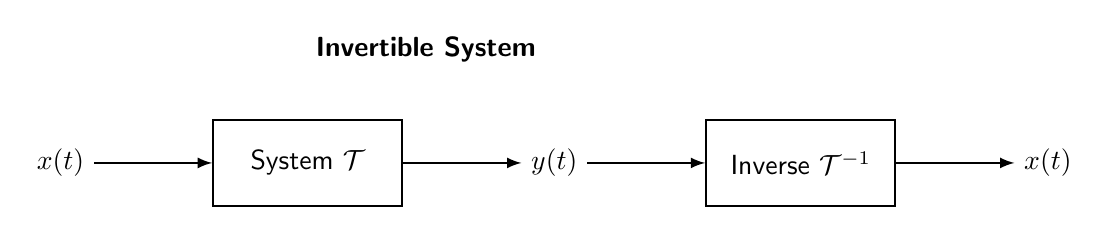
\begin{tikzpicture}[
	% --- STYLES (Unified for a consistent look) ---
	node distance=1.2cm and 1.5cm,
	% A single, modern block style for both parts of the diagram
	block/.style={
		draw, 
		thick,
		minimum height=1.1cm, 
		minimum width=2.4cm, 
		align=center,
		font=\sf
	},
	% The original, reliable line style for arrows
	line/.style={
		-latex, 
		thick
	},
	% Style for plain text nodes to ensure font consistency
	io/.style={
		font=\sf
	}
	]
	

	
	% --- Nodes (using original placement) ---
	\node[io] (in_a) {\(x(t)\)};
	\node[block, right=of in_a] (sys_a) {System \(\mathcal{T}\)};
	\node[io, right=of sys_a] (mid_a) {\(y(t)\)};
	\node[block, right=of mid_a] (inv_a) {Inverse \(\mathcal{T}^{-1}\)};
	\node[io, right=of inv_a] (out_a) {\(x(t)\)};
	
	% --- Connections ---
	\draw[line] (in_a) -- (sys_a);
	\draw[line] (sys_a) -- (mid_a);
	\draw[line] (mid_a) -- (inv_a);
	\draw[line] (inv_a) -- (out_a);
	
	% --- Title ---
	\node[above=0.6cm of sys_a, xshift=1.5cm, font=\sf\bfseries] {Invertible System};
	
	
	
\end{tikzpicture}

		\label{fig:invertibility}
	\end{figure}
	
	\subsection*{3. Causality}
	\begin{definition}
		A system is \textbf{causal} if its output at time \(t_0\) depends only on the input at the same or previous time  \(\{x(t): t \le t_0\}\). Otherwise, it is \textbf{non-causal}.
	\end{definition}
	
	\begin{remark}
		All real-time physical systems must be causal, as they cannot react to future events.
	\end{remark}
	
	\begin{example}
		
		\begin{itemize}[noitemsep]
			\item[]
			\item \( y(t) = x(t - t_0) \) \quad ( \( t_0 \ge 0 \))
			\item \( y[n] = x[2n] \)
			\item \( y(t) = \int_{t}^{t+t_0} x(\tau)\,d\tau \) \quad ( \( t_0 > 0 \))
			\item \( y(t) = x(-2t) \)
			\item \( y(t) = \int_{-\infty}^{t} x(\tau)\,d\tau \)
			\item \( y[n] = \sum_{k=-\infty}^{n} x[k] \)
			\item \( y[n] = x[n-1] \)
			\item \( y(t) = x(t+1) \)
			\item \(
			y(t) = \begin{cases} 
				x(3t) & \text{if } t < 0 \\
				x(t-1) & \text{if } t \geq 0
			\end{cases}
			\)
		\end{itemize}
	\end{example}
	
	
	\subsection*{4. Stability}
	\begin{definition}[BIBO Stability]
		A system is \textbf{Bounded-Input, Bounded-Output (BIBO) stable} if every bounded input produces a bounded output.
	\end{definition}
	
	\begin{example}
		\begin{itemize}
			\item[]
			\item \textbf{Stable Systems:} A bounded input $|x| \le B_x$ produces a bounded output $|y| \le B_y$.
			\begin{itemize}[noitemsep]
				\item \textbf{Time Delay:} \( y[n] = x[n-1] \). A simple shift does not alter the amplitude bounds of the signal. Stable.
				\item \( y(t) = \int_{t}^{t+t_0} x(\tau)\,d\tau \). The output is bounded by \(|y(t)| \le |t_0| \cdot B_x\). Stable.
				\item \textbf{Moving Average:} \( y[n] = \frac{1}{2M+1}\sum_{k=-M}^{M} x[n-k] \). The output is bounded by \(|y[n]| \le B_x\). Stable.
				\item  \( y(t) = e^{x(t)} \). If \(|x(t)| \le B_x\), the output is bounded by \(|y(t)| \le e^{B_x}\). Stable.
			\end{itemize}
			\vspace{0.2cm}
			\item \textbf{Unstable Systems:} A bounded input can produce an unbounded output.
			\begin{itemize}[noitemsep]
				\item \textbf{Differentiator:} \( y(t) = \frac{d}{dt}x(t) \). A bounded input like \(x(t) = \sin(t^2)\) produces an unbounded output \(y(t) = 2t\cos(t^2)\). Unstable.
				\item \textbf{Integrator:} \( y(t) = \int_{-\infty}^{t} x(\tau)\,d\tau \). The bounded input \(x(t)=u(t)\) produces the unbounded ramp output \(y(t)=t \cdot u(t)\). Unstable.
				\item \textbf{Accumulator:} \( y[n] = \sum_{k=-\infty}^{n} x[k] \). The bounded input \(x[n]=u[n]\) produces the unbounded output \(y[n]=(n+1)u[n]\). Unstable.
			\end{itemize}
		\end{itemize}
	\end{example}
	
	\subsection*{5. Time-Invariance}
	\begin{definition}
		A system is \textbf{time-invariant} if a time shift in the input results in an identical time shift in the output:
		\[
		y(t) = \T\{x(t)\} \implies y(t - t_0) = \T \{ x(t - t_0) \} \quad \forall t_0.
		\]
	\end{definition}
	
	\begin{figure}[H]
		\centering
		
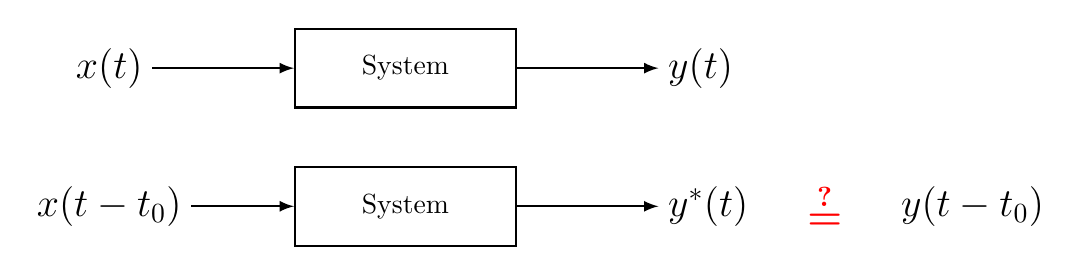
\begin{tikzpicture}[
	node distance=1.5cm and 1.8cm, % Adjust distances as needed
	block/.style={draw, rectangle, minimum width=2.8cm, minimum height=1cm, align=center, thick},
	label_style/.style={font=\Large},
	arrow/.style={-latex, thick}
	]
	
	% --- Top Row: Establishes the baseline system response ---
	\node[label_style] (input_x) {$x(t)$};
	\node[block, right=of input_x] (system_top) {System};
	\node[label_style, right=of system_top] (output_y) {$y(t)$};
	
	% Arrows for top row
	\draw[arrow] (input_x) -- (system_top);
	\draw[arrow] (system_top) -- (output_y);
	
	
	% --- Bottom Row: Poses the time-invariance question ---
	% Position this row below the top one
	\node[label_style, below=1cm of input_x] (input_x_shifted) {$x(t-t_0)$};
% Align the bottom system block vertically with the top one
\node[block] (system_bottom) at (system_top |- input_x_shifted) {System};
	\node[label_style, right=of system_bottom] (output_y_prime) {$y^*(t)$};
	
	% --- The key illustrative question ---
	\node[label_style, right=0.5cm of output_y_prime, text=red] (question) {$\boldsymbol{\stackrel{?}{=}}$};
	\node[label_style, right=0.5cm of question] (final_output) {$y(t-t_0)$};
	
	
	% Arrows for bottom row
	\draw[arrow] (input_x_shifted) -- (system_bottom);
	\draw[arrow] (system_bottom) -- (output_y_prime);
	
\end{tikzpicture}
		\caption{Time-invariance principle: shifting input shifts output.}
		\label{fig:time_invariance_block}
	\end{figure}
	
	\begin{remark}
		Physical systems whose properties do not change over time are time-invariant (e.g., an RC circuit with fixed component values).
	\end{remark}
	
	\begin{example}
		\vspace{0.5em}
		\begin{itemize}[noitemsep]
			\item[]
			\item \( y(t) = x(t + f(t)) \)
			\item \( y(t) = \frac{d}{dt}x(t) \)
			\item \( y(t) = f(x(t)) \)
			\item \( y(t) = x(f(t)) \)
			\item \( y(t) = A x(t + \alpha) \)
			\item \( y(t) = A x(\alpha t) \)
		\end{itemize}
	\end{example}
	
	
	\subsection*{6. Linearity}
	\begin{definition}[Linearity]
		A system is \textbf{linear} if it satisfies superposition principles. This combines two properties:
		\begin{enumerate}[noitemsep]
			\item \textbf{Additivity:} \(\T\{x_1 + x_2\} = \T\{x_1\} + \T\{x_2\}\).
			\item \textbf{Homogeneity (Scaling):} \(\T\{\alpha x\} = \alpha \T\{x\}\), for any scalar \(\alpha \in \C\).
		\end{enumerate}
		The two properties can be combined into a single statement:
		\[\T\{\alpha x_1 + \beta x_2\} = \alpha \T\{x_1\} + \beta \T\{x_2\}\]
		for any inputs \(x_1, x_2\) and any scalars \(\alpha, \beta \in \C\).
	\end{definition}
	
	\captionsetup[figure]{labelformat=empty}
	\begin{figure}[H]
		\centering
		
	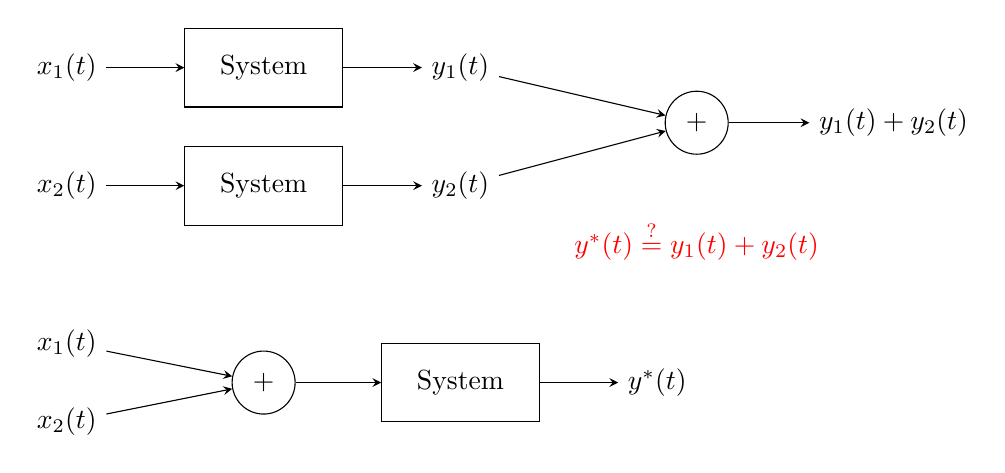
\begin{tikzpicture}[
		block/.style={rectangle, draw, minimum width=2cm, minimum height=1cm, align=center},
		sum/.style={circle, draw, minimum size=0.8cm, align=center},
		node distance=2.5cm,
		>=stealth
		]
		
		% Top row - Individual systems
		% First path: x1(t) -> System -> y1(t)
		\node (x1) {$x_1(t)$};
		\node[block, right of=x1] (sys1) {System};
		\node[right of=sys1] (y1) {$y_1(t)$};
		
		% Second path: x2(t) -> System -> y2(t)  
		\node[below of=x1, node distance=1.5cm] (x2) {$x_2(t)$};
		\node[block, right of=x2] (sys2) {System};
		\node[right of=sys2] (y2) {$y_2(t)$};
		
		% Bottom row - Combined system
		% Input summing junction
		\node[below of=x2, node distance=2cm] (x1_bottom) {$x_1(t)$};
		\node[below of=x1_bottom, node distance=1cm] (x2_bottom) {$x_2(t)$};
		\node[sum, right of=x1_bottom, yshift=-0.5cm] (sum_input) {$+$};
		\node[block, right of=sum_input] (sys_combined) {System};
		\node[right of=sys_combined] (y_prime) {$y^*(t)$};
		
		% Right side - Comparison and output summing
		\node[sum, right of=y1, node distance=3cm,yshift=-0.7cm] (sum_output) {$+$};
		\node[right of=sum_output] (sum_result) {$y_1(t) + y_2(t)$};
		
		% Comparison question
		\node[below of=sum_output, node distance=1.5cm , red] (comparison) {$y^*(t) \stackrel{?}{=} y_1(t) + y_2(t)$};
		
		% Arrows for top row
		\draw[->] (x1) -- (sys1);
		\draw[->] (sys1) -- (y1);
		\draw[->] (x2) -- (sys2);
		\draw[->] (sys2) -- (y2);
		
		% Arrows for bottom row
		\draw[->] (x1_bottom) -- (sum_input);
		\draw[->] (x2_bottom) -- (sum_input);
		\draw[->] (sum_input) -- (sys_combined);
		\draw[->] (sys_combined) -- (y_prime);
		
		% Arrows for output summing
		\draw[->] (y1) -- (sum_output);
		\draw[->] (y2) -- (sum_output);
		\draw[->] (sum_output) -- (sum_result);
		
		
	\end{tikzpicture}


		\caption{Additivity principle for linear systems.}
		\label{fig:additivity}
	\end{figure}
	\captionsetup[figure]{labelformat=default}
	
	\begin{figure}[H]
		\centering
		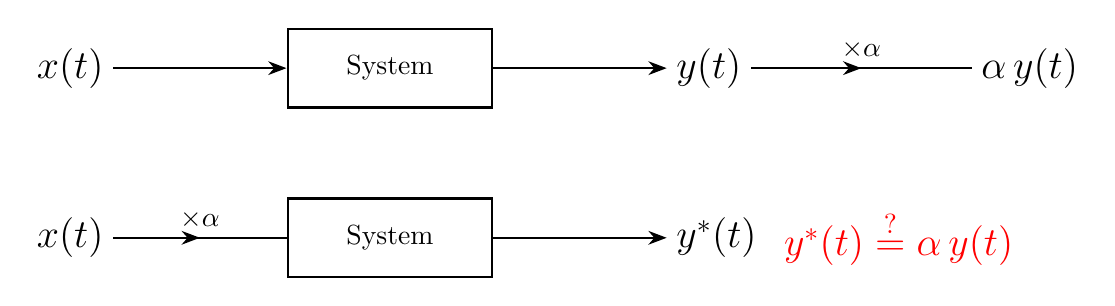
\begin{tikzpicture}[
	node distance = 14mm and 22mm,
	% Styles
	block/.style = {draw, rectangle, minimum width=26mm, minimum height=10mm, align=center, thick},
	sig/.style = {font=\Large}, % Corrected this line
	end arrow/.style = {->, thick, -{Stealth}},
	gain arrow/.style args={#1}{thick, postaction={decorate},
		decoration={markings, mark=at position 0.5 with {
				\arrow{Stealth}; \node[above, inner sep=3pt] {#1};
	}}}
	]
	
	% Top row: base response
	\node[sig] (x) {$x(t)$};
	\node[block, right=of x] (sys) {System};
	\node[sig, right=of sys] (y) {$y(t)$};
	
	% --- CORRECTED Bottom row positioning ---
	% Start the row
	\node[sig, below=of x] (xb) {$x(t)$};
	% Position the rest of the row relative to the node before it
	\node[block, right=of xb] (sysb) {System};
	\node[sig, right=of sysb] (yb) {$y^*(t)$};
	
	% Right side: scaled output
	\node[sig, right=28mm of y] (ay) {$\alpha\,y(t)$};
	
	% Comparison question
	\node[sig, red, right=1mm of yb] (cmp) {$y^*(t)\stackrel{?}{=} \alpha \,y(t)$};
	
	% Paths
	\draw[end arrow] (x) -- (sys);
	\draw[end arrow] (sys) -- (y);
	
	% This arrow will now be perfectly straight
	\draw[gain arrow={$\times \alpha$}] (xb) -- (sysb);
	
	\draw[end arrow] (sysb) -- (yb);
	
	\draw[gain arrow={$\times \alpha$}] (y) -- (ay);

	
\end{tikzpicture}
		\caption*{Homogeneity scaling principle for linearity.}
		\label{fig:homogeneity}
	\end{figure}
	
	\begin{remark}
		A necessary (but not sufficient) condition for linearity is that a zero input must produce a zero output: \(\T\{0\}=0\).
	\end{remark}
	\newpage
	\begin{example}
		\begin{itemize}
			\item \textbf{Linear Systems:} Obey the superposition principle $\T\{ax_1 + bx_2\} = a\T\{x_1\} + b\T\{x_2\}$.
			\begin{itemize}[noitemsep]
				\item \( y(t) = A x(\alpha t + \beta) \): Time scaling, shifting, and amplitude scaling are all linear operations.
				\item \( y(t) = \frac{d}{dt}x(t) \): Differentiation is a linear operator.
				\item \( y(t) = \int_{-\infty}^{t} x(\tau)\,d\tau \): Integration is a linear operator.
				\item \( y[n] = \sum_{k=-\infty}^{n} x[k] \): Summation is a linear operator.
				\item \( y(t) = x(f(t)) \): \textbf{(Linear)} The transformation is on the time variable, not the signal's amplitude.
				\item \( y(t) = x(t+f(t)) \): \textbf{(Linear)} Similar to the above, this is a time-varying shift, which is a linear operation.
			\end{itemize}
			\vspace{0.2cm}
			
			\item \textbf{Non-Linear Systems:} Violate either additivity or homogeneity.
			\begin{itemize}[noitemsep]
				\item \( y[n] = x[n-1]x[n] \): Fails homogeneity, as scaling the input by $a$ scales the output by $a^2$.
				\item \( y[n] = x[n] + C \): Fails the zero-input test; if $x[n]=0$, $y[n]=C \neq 0$.
				\item \( y(t) = |x(t)| \): Fails homogeneity, since $|-x(t)| = |x(t)| \neq -|x(t)|$.
				\item \( y(t) = \Re\{x(t)\} \): Fails homogeneity for complex scalars (e.g., $\Re\{j \cdot 1\} = 0$, but $j \cdot \Re\{1\} = j$). It is, however, additive.
				\item \( y[n] = \Im\{x[n]\} \): Also fails homogeneity for complex scalars.
				\item \( y(t) = x^*(t) \): The complex conjugate fails homogeneity for complex scalars, since $(ax(t))^* = a^*x^*(t) \neq ax^*(t)$.
				\item \( y(t) = x(t) + f(t) \): Fails the zero-input test if $f(t) \neq 0$.
			\end{itemize}
		\end{itemize}
	\end{example}
	
\section*{3.3 Summary and Next Lecture}
	\begin{itemize}[noitemsep]
		\item Defined systems and six fundamental properties: memory, invertibility, causality, stability, time-invariance, and linearity.
		\item System interconnections: series, parallel, and feedback.
		\item Linear Time-Invariant (LTI) systems are most important for analysis.
		\item \textbf{Next time:} LTI system characterization and convolution.
	\end{itemize}
	
\end{document}